\chapter{Asking Millionaires How They Got Rich: Houston}

This chapter is a study in commercial rather than formal mathematics. We are not given a blackboard full of symbols; we are given a sequence of operating cases, each with just enough arithmetic to ask a sharp question: when does income turn into wealth? We follow the lecture in its own order. First comes the numerical tease, then the interviews, then the increasingly explicit rules: hold money, survive losses, align incentives, deploy capital, and sell oneself before selling anything else.

\section{Revenue First, Explanation Later}

The lecture opens on a puzzle. A restaurant owner says he occupies only \(4600\) square feet and nevertheless did one million dollars of revenue in a single month. Only after this do we widen to Houston as a city dense with millionaires. The order matters. We are not first given a philosophy of wealth; we are first given a number large enough to demand an explanation.

We begin by assigning notation to the opening teaser. Let \(A\) be the restaurant footprint, \(R_{\mathrm{mo}}\) the one-month revenue, and \(\rho_{\mathrm{mo}}\) the monthly revenue density:
\begin{equation}
A=4600\ \text{sq ft},
\qquad
R_{\mathrm{mo}}=1{,}000{,}000\ \text{USD}.
\end{equation}
Then
\begin{equation}
\rho_{\mathrm{mo}}
=
\frac{R_{\mathrm{mo}}}{A}
=
\frac{1{,}000{,}000}{4600}
\approx
217.4\ \text{USD}\,\text{sq ft}^{-1}\,\text{month}^{-1}.
\end{equation}

This is not yet the central lesson of the chapter. It is the bait. The lecture will spend the rest of its time explaining what kinds of decisions, habits, and operating structures can sit behind such a number.

\section{Making Money and Keeping Money}

The first interview gives us a speaker in the concierge space: private jet charter, yacht charter, exotic cars, the whole luxury-service package. The reported earnings are large, somewhere between \(2.5\) and \(5\) million dollars in a year. Just as important, the host does not stop at the income figure. He asks for the best financial decision of a lifetime, and the answer is much more severe than the earnings number: learn to hold on to money.

\begin{definition}
We shall use the editorial bookkeeping symbols
\begin{equation}
K_t = Y_t - C_t - L_t,
\end{equation}
where \(Y_t\) is income earned in period \(t\), \(C_t\) is consumption or cash leakage, and \(L_t\) is loss absorption. We then define deployable wealth recursively by
\begin{equation}
W_{t+1}=W_t+K_t.
\end{equation}
\end{definition}

The lecture does not write these symbols on a board, but this is exactly the structure of the claim. A person may have a large \(Y_t\) and still fail to increase \(W_t\) if \(C_t\) and \(L_t\) drain the surplus.

\subsection{Question \& Answer}

\paragraph{Question.} Why does high income fail so often to become wealth?

\paragraph{Answer.} Because the decisive object is not gross earnings but retained capital. The interviewee's point is that many people can make money, but not many can keep it. In our notation, the danger is not a small \(Y_t\); it is a small or vanishing \(K_t\).

The same interview gives another important, if slightly garbled, maxim: keep the right people around you. Even here, the lecture is already tying money to social structure. Wealth is not shown as a solitary act of cleverness. It appears through networks, trust, and access to high-value transactions, but it survives only if the surplus is retained.

The host then pauses and recaps. That pause matters. It tells us that the first interview is meant to function as a principle, not merely as a biographical curiosity: high earnings are flashy; retention is decisive.

\begin{figure}
\centering
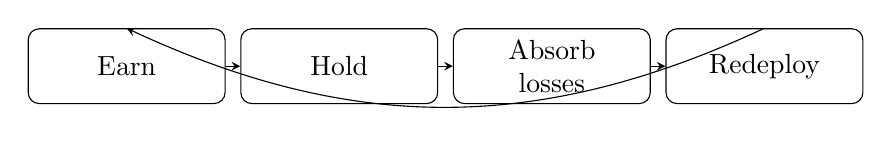
\begin{tikzpicture}[>=stealth, node distance=2.7cm, every node/.style={draw, rounded corners, minimum width=2.5cm, minimum height=0.95cm, align=center}]
\node (earn) {Earn};
\node (hold) [right of=earn] {Hold};
\node (loss) [right of=hold] {Absorb\\losses};
\node (redeploy) [right of=loss] {Redeploy};
\draw[->] (earn) -- (hold);
\draw[->] (hold) -- (loss);
\draw[->] (loss) -- (redeploy);
\draw[->, bend left=25] (redeploy.north) to (earn.north);
\end{tikzpicture}
\caption{Editorial schematic of the lecture's recurrent capital recursion: earn, retain, absorb losses, redeploy, and begin again.}
\end{figure}

\section{Career Redirection and the First-Business Problem}

The second long interview begins with redirection. We move from computer science to biology, from there to medicine, and then from medicine into real estate and business. The lecture is careful here. It does not present passion as a fixed early truth. Instead it allows a path to bend: a job may be worth having long enough to learn from it, and then one moves.

That biographical flexibility sets up a harder economic point. When the host asks about peak earnings, the answer is deliberately two-sided: there were years of losses, and there were good years around \(4\) to \(5\) million dollars. Those good years were used to offset earlier losses and then to reinvest into growth.

\paragraph{A worked update rule.} The logic can be written in short steps:
\begin{enumerate}
\item Early years may have \(L_t>Y_t\), so net capital creation is negative.
\item Later profitable years may have \(Y_t\in [4,5]\) million USD.
\item The first call on those profits is not celebration but repair: prior losses must be offset.
\item Only the residual enters new growth, that is, only after loss absorption do we obtain positive \(K_t\) fit for redeployment.
\end{enumerate}

This is the first place where the lecture becomes stern. The speaker says the first business is always the hardest, that it took years to make profitable, and that there were stretches of ninety-six hours straight. One can hear the transition from romance to operating reality.

\subsection{Question \& Answer}

\paragraph{Question.} Why is the first business so hard?

\paragraph{Answer.} The answer given here is not merely that it is time-consuming. It is that the first business forces an operator to exchange ego for correction. When something fails, one does not win by locating blame elsewhere. One wins by asking: how could I have hired better, trained better, or motivated better?

In this way the lecture turns accountability into a correction loop:
\begin{equation}
\text{failure}
\longrightarrow
\text{self-audit}
\longrightarrow
\text{better hiring/training/motivation}
\longrightarrow
\text{corrected operation}.
\end{equation}

We then move, almost naturally, from business failure to investment caution. If nearly everybody will try to take advantage of the novice, then the first duty of a young earner is not to hand capital away. Save first. Delay the visible consumption that kills later optionality. The lecture's point is almost austere: if the money is spent too quickly, there will be nothing left when a genuine opportunity appears.

A brief marine-industry interlude follows, with a simple exhortation to follow one's dreams and remember that life is finite. In the architecture of the lecture this is less a new theorem than a breathing point. It resets the rhythm before the densest case of the chapter.

\section{The Restaurant as a Worked Operating Model}

Now the lecture returns to the teaser and finally pays it off. We enter one of the most popular restaurants in Houston and speak to the owner. This is the chapter's central operating case because it combines origin story, unit economics, incentive design, governance, owner presence, and service policy.

The origin story is modest. The owner says he started waiting tables at sixteen and worked upward. That matters because the later numbers are not presented as magic. They are presented as the result of extreme immersion in one operating environment.

\paragraph{Anecdote.} The owner says he is working out of a \(4600\)-square-foot restaurant, that in December he did one million dollars in revenue in a single month, and that the full year came in just under \(10\) million.

\paragraph{Claim.} The claim is not merely that the restaurant is popular. It is that the business achieves exceptional revenue density.

\paragraph{Mechanism.} The mechanisms are several: constant owner presence, incentive alignment for key employees, paperwork, decision clarity with partners, relentless communication, and a premium service model in which the answer is never a flat no.

Let \(R_{\mathrm{yr}}\) denote the full-year revenue. Then the annual density is
\begin{equation}
\rho_{\mathrm{yr}}
=
\frac{R_{\mathrm{yr}}}{A}
\approx
\frac{10{,}000{,}000}{4600}
\approx
2173.9\ \text{USD}\,\text{sq ft}^{-1}\,\text{year}^{-1}.
\end{equation}
If we annualize the one-month teaser run rate, we obtain
\begin{equation}
\rho_{\mathrm{yr}}^{(\mathrm{annualized\ teaser})}
=
12\,\rho_{\mathrm{mo}}
\approx
2608.7\ \text{USD}\,\text{sq ft}^{-1}\,\text{year}^{-1}.
\end{equation}

The owner also says ``\(2300\) to \(2400\) a square foot.'' The numbers do not line up perfectly if we treat every spoken quantity as exact. We therefore keep the statement as reported and note only that the annual density computed from ``just under \(10\) million'' lies nearby, while the annualized teaser month lies above it. The lecture's point survives the numerical tension: this is an unusually dense revenue machine.

\subsection{Question \& Answer}

\paragraph{Question.} How can a \(4600\)-square-foot restaurant produce such outsized revenue?

\paragraph{Answer.} The lecture answers this by stacking mechanisms rather than by giving a single formula. We have density of demand, density of service, density of management, and density of incentive. The owner is there constantly. He knows the customers. He touches every table. He ties key employees to outcomes. He makes decisions legible on paper. And he refuses to let the service experience collapse into the word ``no.''

That last point is economic, not merely theatrical. The owner gives a striking example: if a guest wants a car delivered from the Rolls-Royce dealer, he will source it, add twenty percent to the check, and make it happen. If \(P_{\mathrm{source}}\) is the acquisition cost and \(P_{\mathrm{client}}\) the billed customer price, then the policy is
\begin{equation}
P_{\mathrm{client}}=(1+m)P_{\mathrm{source}},
\qquad
m=0.20.
\end{equation}
This is a miniature pricing rule for premium service: not refusal, but fulfillment with markup.

The incentive structure is equally clear. The owner tells key employees that if the business reaches its year-end number, he will write a check, sometimes \(5000\), sometimes \(10{,}000\). We may write this as a threshold rule
\begin{equation}
B_i=
\begin{cases}
b_i, & \text{if the target }T\text{ is reached},\\
0, & \text{otherwise},
\end{cases}
\qquad
b_i\in\{5000,10000\}\ \text{USD}.
\end{equation}

Partnership structure is treated with equal seriousness. Get everything in writing. If there are partners, there must be a decision maker. Communication is key. One can hear the lecture moving from glamorous revenue numbers back into administrative bone and connective tissue. Here again we are told that wealthy people invest in people, not in abstractions. Presence is part of the asset.

The host then recaps with open admiration. We should keep that admiration in the notes, not as hype, but as a signal that this case is the lecture's center of gravity.

\section{Where Surplus Cash Goes}

After the restaurant sequence, the lecture pivots from operating excellence to capital deployment. We begin with a real-estate investor who also owns restaurants and a shipping-container park. The advice is concrete: get into areas that are beginning to gentrify, but get there early. Watch where experienced investors are already moving. Watch for schools, new HEBs, Amazon-centered development, and similar signals of fresh demand.

This is not a theorem. It is a field heuristic. But it has a distinct logical structure. One looks for underpriced land before the consensus arrives. One reads institutional and infrastructural signals. One follows credible builders without merely imitating the crowd. One starts before feeling perfect.

The next speakers extend the point. One says the crucial step is to think about growing one's own business rather than remaining indefinitely an employee. Another, who moved after twenty-three years of employment into a propane-export business, says the core of life is relationships. Another entrepreneur, moving through sales, mortgages, and eventually a company serving fine restaurants, says he would have raised capital and surrounded himself with really good people from day one.

\paragraph{A compact ledger of cases.}
\begin{itemize}
\item Concierge business: \(2.5\) to \(5\) million USD per year; the governing rule is to keep money once earned.
\item Doctor turned operator: good years of \(4\) to \(5\) million USD; the governing rule is to offset losses before redeploying.
\item Restaurant owner: roughly \(10\) million USD per year at \(4600\) square feet; the governing rule is density plus presence plus incentives.
\item Real-estate operator: roughly \(2\) million USD per year; the governing rule is to enter promising areas early.
\item Medical sales: roughly \(400{,}000\) to \(500{,}000\) USD per year; the governing rule is to sell oneself through service.
\end{itemize}

\subsection{Question \& Answer}

\paragraph{Question.} Once surplus cash exists, where should it go first, and what should remain liquid?

\paragraph{Answer.} The lecture offers an ordered heuristic rather than a universal law. Real estate is named first. But before one becomes too clever, one should hold a cash cushion of roughly six to twelve months of spend. Only after that does the lecture move toward broad-market equity exposure through the S\&P 500.

In symbols, if \(S_{\mathrm{mo}}\) is monthly spend, then the recommended buffer is
\begin{equation}
B_{\mathrm{cash}} \in [6,12]\;S_{\mathrm{mo}}.
\end{equation}
One may therefore think of the allocation ladder as
\begin{enumerate}
\item preserve capital by not spending too early;
\item build liquidity \(B_{\mathrm{cash}}\);
\item deploy into real estate;
\item use broad-market equity exposure, here named as the S\&P 500, for the remainder.
\end{enumerate}

The lecture then turns more philosophical without losing its economic edge. If Warren Buffett prefers the index over the fantasy of beating every expert, why should the novice imagine himself smarter than the field? The same logic appears in the ``do not be a sheep'' analogy. One should not automatically join the crowded lane simply because it is crowded. This is not formal decision theory. It is a warning against default imitation.

\section{Sales, Self-Investment, and the Portability of Skill}

The last stretch narrows the field once more. We meet a medical salesperson doing foot-and-ankle implant sales, earning roughly \(400{,}000\) to \(500{,}000\) dollars in a year. The advice is familiar by now and yet sharpened by the sales context: push yourself, do not say no, keep showing the customer your service, and remember that in sales the person is often buying you.

This turns the earlier restaurant logic into a more general rule. Customer service, commitment, and follow-through are not ornaments; they are part of the product. When the speaker says one never stops investing in oneself and never stops investing in real estate, the lecture joins inner capital to outer capital. The asset is partly the property portfolio and partly the operator who can continue to earn, persuade, and execute.

The engineering interview complicates rather than cancels the entrepreneurial line. One speaker says that, in his case, the right move was college and an engineering degree. But when the host asks whether a college degree is necessary in general, the answer is no: it depends on skill set. This is faithful to the chapter's larger method. There is no one path, but there are recurring structures.

The final real-estate pair drives the chapter to its closing portable rule. Sell yourself first. If people like you, they buy from you. Ask enough questions and people will, in effect, sell themselves on your offer. Thus the lecture ends not with a single industry secret but with a trans-industry discipline: the ability to sell oneself, communicate, and build trust.

\subsection{Question \& Answer}

\paragraph{Question.} What skill survives across all these industries?

\paragraph{Answer.} The lecture's final answer is that the portable skill is not a single product competence. It is the ability to sell oneself through questions, service, presence, and trust. One can be an accountant, an engineer, a doctor, a restaurateur, or a real-estate operator; but if one cannot persuade, one cannot compound opportunity.

\section{Summary}

We may now state the chapter in the lecture's own order. It begins with a startling revenue number, then asks how such numbers arise, and finally asks what remains after spending, losses, and bad deployment are stripped away. The answer is not one formula but a family of operating rules.

We earn. We hold. We absorb losses. We redeploy. We compound. Along the way we learn that partnerships need paperwork, incentives need thresholds, service can justify markup, real-estate investing rewards early observation, and cash buffers protect later freedom. Above all, the lecture insists that wealth is not merely made; it is retained, governed, and directed. That is the commercial mathematics of the episode.